Исследуем подробно поведение траекторий в окрестности точки покоя линейной системы
\begin{equation*}
    \dot{r} = Ar
\end{equation*}
если $A \in M_2(\mathbb{R})$. Пусть $\det A \neq 0$, тогда имеется единственное положение равновесия $r = 0$ и собственные числа $\lambda_1, \lambda_2$ матрицы $A$ отличны от нуля.\\

\noindent \textbf{Случай $\lambda_1, \lambda_2 \in \mathbb{C}$, $Im\, \lambda_{1,2} \neq 0$}

Поскольку матрица $A$ вещественная, то $\lambda_1 = \overline{\lambda_2}$. Пусть $\lambda = \lambda_1$, $h$ --- соответствующий собственный вектор. Тогда $Re\, h$, $Im\, h$ --- базис в $\mathbb{R}^2$. Поскольку
\begin{equation*}
    Re\, h = \frac{h + \overline{h}}{2}, \quad Im\, h = \frac{h - \overline{h}}{2i} = \frac{-ih + i\overline{h}}{2}
\end{equation*}
то матрица перехода $T$ к базису $Re\, h$, $Im\, h$ представима в виде
\begin{equation*}
    T = (Re\, h, Im\, h) = \frac{1}{2}(h,\overline{h})
    \begin{pmatrix}
    1 & -i\\
    1 & i
    \end{pmatrix}
\end{equation*}

Пусть $H = (h, \overline{h})$ --- матрица перехода к собственному базису. Подставляя $r = Ts$ в уравнение $\dot{r} = Ar$, находим
\begin{equation*}
    \frac{1}{2}H
    \begin{pmatrix}
    1 & -i\\
    1 & i
    \end{pmatrix}
    \dot{s} = A\frac{1}{2}H
    \begin{pmatrix}
    1 & -i\\
    1 & i
    \end{pmatrix}
    s
\end{equation*}
Сокращая на множитель $\frac{1}{2}$ и умножая слева на $H^{-1}$, получаем
\begin{equation}
    \begin{pmatrix}
    1 & -i\\
    1 & i
    \end{pmatrix}
    \dot{s} = H^{-1}AH
    \begin{pmatrix}
    1 & -i\\
    1 & i
    \end{pmatrix}
    s \label{newsyst2}
\end{equation}
Поскольку $H^{-1}AH = diag(\lambda, \overline{\lambda})$, то система (\ref{newsyst2}) имеет вид
\begin{equation*}
    \begin{cases}
    \dot{u} - i\dot{v} = \lambda(u - iv)\\
    \dot{u} + i\dot{v} = \overline{\lambda}(u + iv)
    \end{cases}
\end{equation*}

Уравнения этой системы равносильны: одно получается из другого при комплексном сопряжении. Поэтому достаточно рассмотреть только одно из них. Положим $z = u + iv$. Тогда второе уравнение принимает вид
\begin{equation*}
    \dot{z} = \overline{\lambda}z
\end{equation*}
Его решения $z = Ce^{\overline{\lambda}t}$

Пусть $\lambda = \alpha + i\beta$, $C = ae^{i\varphi}$. Тогда
\begin{equation*}
    z = ae^{\alpha t}e^{i(\varphi - \beta t)}
\end{equation*}

При $\alpha = 0$ получаем окружности радиуса $a$. Соответствующая устойчивая, но не асимптотически устойчивая точка покоя называется \textbf{центр}. Направление обхода окружностей зависит от знака $\beta$.

При $\alpha > 0$ получаем логарифмическую спираль. Модуль $z$ возрастает, значит, точка удаляется от начала координат, при этом совершая вокруг него обороты. Данное положение равновесия называется \textbf{неустойчивый фокус}.

При $\alpha < 0$ спираль закручивается. Точка покоя --- \textbf{устойчивый фокус}. Направление закручивания или раскручивания траекторий в случае фокуса зависит от знака $\beta$ (см. \hyperref[focus]{рисунок}).

\begin{figure}[H]\label{focus}
    \center{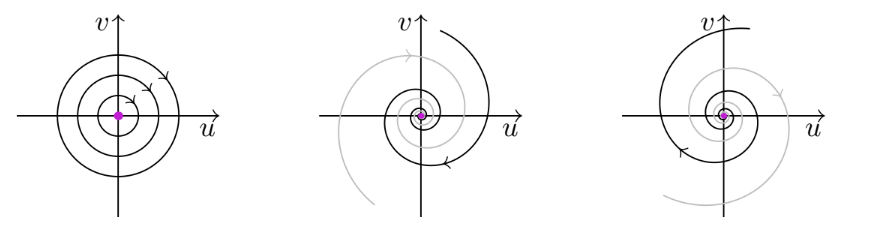
\includegraphics[scale=0.5]{Pics/focus.png}}
    \caption{Центр, устойчивый и неустойчивый фокус}
\end{figure}
